\documentclass{sigchi}


% Load basic packages
\usepackage{balance}       % to better equalize the last page
\usepackage{graphics}      % for EPS, load graphicx instead 
\usepackage[T1]{fontenc}   % for umlauts and other diaeresis
\usepackage{txfonts}
\usepackage{mathptmx}
\usepackage[pdflang={en-US},pdftex]{hyperref}
\usepackage{color}
\usepackage{booktabs}
\usepackage{textcomp}

% Some optional stuff you might like/need.
\usepackage{microtype}        % Improved Tracking and Kerning
% \usepackage[all]{hypcap}    % Fixes bug in hyperref caption linking
\usepackage{ccicons}          % Cite your images correctly!
% \usepackage[utf8]{inputenc} % for a UTF8 editor only

% If you want to use todo notes, marginpars etc. during creation of
% your draft document, you have to enable the "chi_draft" option for
% the document class. To do this, change the very first line to:
% "\documentclass[chi_draft]{sigchi}". You can then place todo notes
% by using the "\todo{...}"  command. Make sure to disable the draft
% option again before submitting your final document.
\usepackage{todonotes}

% Paper metadata (use plain text, for PDF inclusion and later
% re-using, if desired).  Use \emtpyauthor when submitting for review
% so you remain anonymous.
\def\plaintitle{GeoGuessrAI: Image based GeoLocation - Project Proposal}
\def\plainauthor{First Author, Second Author, Third Author,
  Fourth Author, Fifth Author, Sixth Author}
\def\emptyauthor{}
\def\plainkeywords{Authors' choice; of terms; separated; by
  semicolons; include commas, within terms only; this section is required.}
\def\plaingeneralterms{Documentation, Standardization}

% llt: Define a global style for URLs, rather that the default one
\makeatletter
\def\url@leostyle{%
  \@ifundefined{selectfont}{
    \def\UrlFont{\sf}
  }{
    \def\UrlFont{\small\bf\ttfamily}
  }}
\makeatother
\urlstyle{leo}

% To make various LaTeX processors do the right thing with page size.
\def\pprw{8.5in}
\def\pprh{11in}
\special{papersize=\pprw,\pprh}
\setlength{\paperwidth}{\pprw}
\setlength{\paperheight}{\pprh}
\setlength{\pdfpagewidth}{\pprw}
\setlength{\pdfpageheight}{\pprh}

% Make sure hyperref comes last of your loaded packages, to give it a
% fighting chance of not being over-written, since its job is to
% redefine many LaTeX commands.
\definecolor{linkColor}{RGB}{6,125,233}
\hypersetup{%
  pdftitle={\plaintitle},
% Use \plainauthor for final version.
%  pdfauthor={\plainauthor},
  pdfauthor={\emptyauthor},
  pdfkeywords={\plainkeywords},
  pdfdisplaydoctitle=true, % For Accessibility
  bookmarksnumbered,
  pdfstartview={FitH},
  colorlinks,
  citecolor=black,
  filecolor=black,
  linkcolor=black,
  urlcolor=linkColor,
  breaklinks=true,
  hypertexnames=false
}

% create a shortcut to typeset table headings
% \newcommand\tabhead[1]{\small\textbf{#1}}

% End of preamble. Here it comes the document.
\begin{document}

\title{\plaintitle}

\numberofauthors{3}
\author{%
  \alignauthor{Nirvan S.P. Theethira\\
    \affaddr{CSCI6502 001}\\
    \affaddr{Boulder, CO}\\
    \email{nith5605@colorado.edu}}\\
}

\maketitle

\begin{abstract}
  Geolocation can be defined as the identification or estimation of real-world geographic location using location based data. The location based data used for geolocation include but is not limited to satellite images, sensor data, traffic movement data, pollution data etc. Humans are not the best at guessing locations based on sensor data. But when it comes to location based image data, well travelled humans perform fairly well at guessing the location of the image. With google street view, it is now possible to obtain image data from most location in the United States. The game Geoguessr \cite{Geoguessr:Online} presents street view data to human players who attempt to guess the location of the street view image. Using the recent advances in image recognition technology this project aims to emulated and hopefully surpass the scores of human players in the game Geoguessr for the United States map.
\end{abstract}



\section{Motivation}
\begin{figure*}
  \centering
  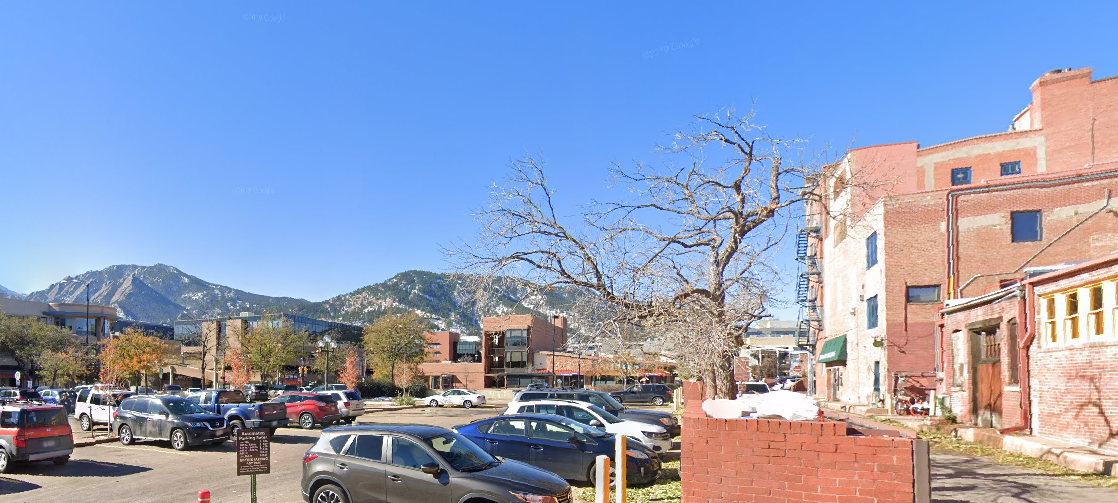
\includegraphics[width=0.6\columnwidth]{figures/perlStreetView.png}
  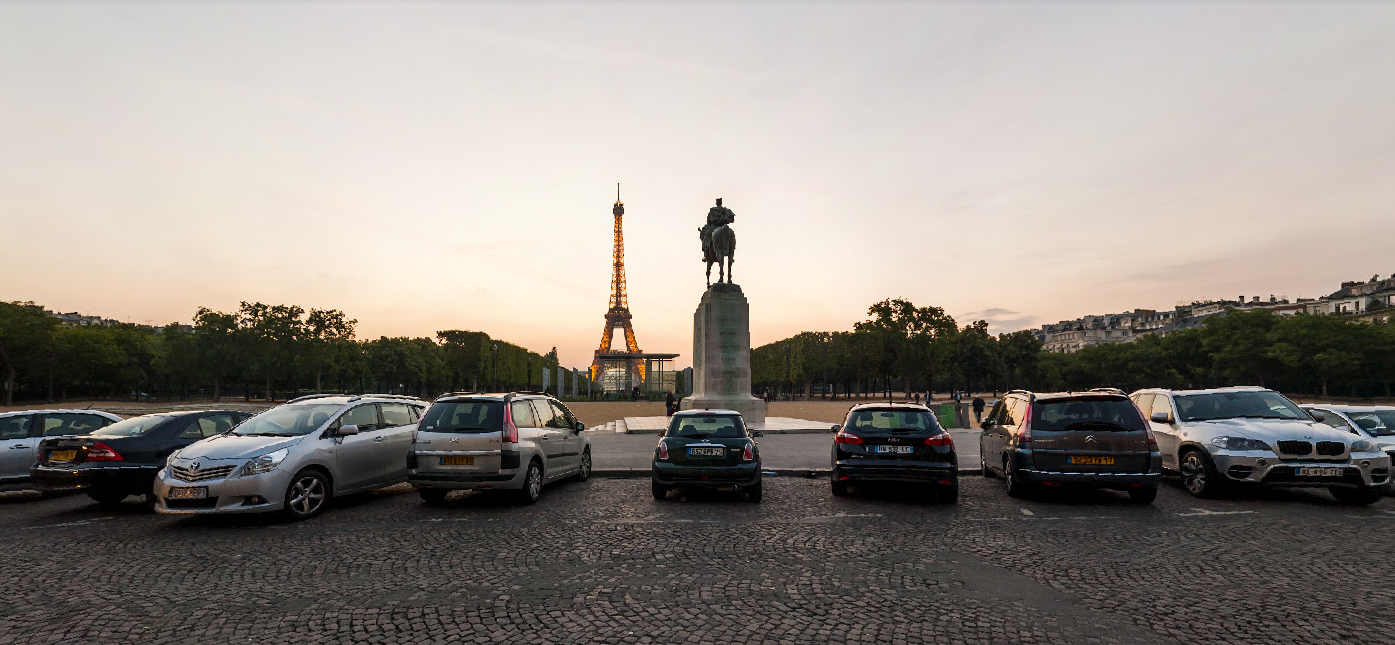
\includegraphics[width=0.6\columnwidth]{figures/eiffle.png}
  \caption{A comparison of a random location (Boulder,CO) on google street view to a famous location (Eiffel Tower) on google street view.}~\label{fig:figure1}
\end{figure*}
The geolocation of a real-world location is the latitude and longitude of that location. One specific application of geolocation would be inferring the location of a tracked animal based, for instance, on the time history of sunlight brightness or the water temperature and depth measured by an instrument attached to the animal. While this is a useful, real world application, the ability to just use images to identify a location would greatly help in a myriad of tasks. The ability to geolocate images can help in geotagging new unseen data thereby facilitation the creation of new dataset. Another application of this technology could be to aid in identifying location with low or no connectivity. A person who is lost in a low connectivity region could snap an image of the surroundings to get an estimate of their location. \\
The motivation for this project comes form the game called Geoguessr \cite{Geoguessr:Online}. The game presents players with street view images (see Figure~\ref{fig:figure1}) which the user, using any pre-existing knowledge, has to guess the location of the image. The use of pre existing knowledge offers well travelled players an advantage in the game. Prior knowledge may include the use of language on street signs, motor vehicle type or in some instances the fact that certain regions (military bases) cannot be reached by google maps can help in elimination of those locations. The game scores the user based on how closed the latitude an longitude of the guess was to the actual latitude and longitude of the location of the street view image. While this is an extremely challenging task for a machine that has no prior knowledge that a avid traveller possess, the use of CNN's for other image recognition tasks have given astonishing results. While previous projects have aimed to geolocate prominent landmarks of locations such as the Eiffle tower, The Taj Mahal etc. this project  aims to use generic images to extract locations. While humans can use prior knowledge as mentioned above, most humans who play the game use geographic features such as building styles, vegetation, mountains, weather etc to find locations. With the plethora of street view images available, a deep neural network can learn to notice these subtleties. As seen in Figure~\ref{fig:figure1} on the left image, there are mountains and red stone buildings which can be used by a deep neural network to ascertain if the image is from boulder. 

\section{Related Work}
There are three main approaches that have been researched:
\begin{itemize}
    \item There are a few already existing approaches for the above mentioned task. One of the elementary approaches deals with the unsupervised k-NN algorithm \cite{Hays:2008:im2gps}. It uses the clustering algorithm to cluster similar images. This idea is used to cluster images from a single location into a single cluster. A new image is run through the K-NN algorithm to find how close the image is to the centroids of the location cluster. The sofmax of these distances denotes how likely the image is from a particular location.
    \item There has been drastic improvements in the field of image recognition with the use of ResNet \cite{DBLP:journals/corr/HeZRS15}. The next method therefore uses the CNN to geolocate images \cite{DBLP:journals/corr/WeyandKP16}. For the dataset, geotagged images scraped from Flickr was used in training and testing. One drawback of using Flickr images is that it results in indoor images and image of people that could clutter the dataset during training. The entire map is split into grids and images are collected from each grid. The model is trained to give a soft maxed output across the grids (see Figure~\ref{fig:figure3}).
    \item The third method takes into account that multiple images can be used in a single classification \cite{DBLP:journals/corr/WeyandKP16}. To process multiple images in one training epoch, the list of images are fed into CNN's that give the vector representations of the list of images. These vectors are then fed into a sequential LSTM and the output is soft maxed across regions from which data is collected (see Figure~\ref{fig:figure3}).
\end{itemize}
\begin{figure*}
  \centering
  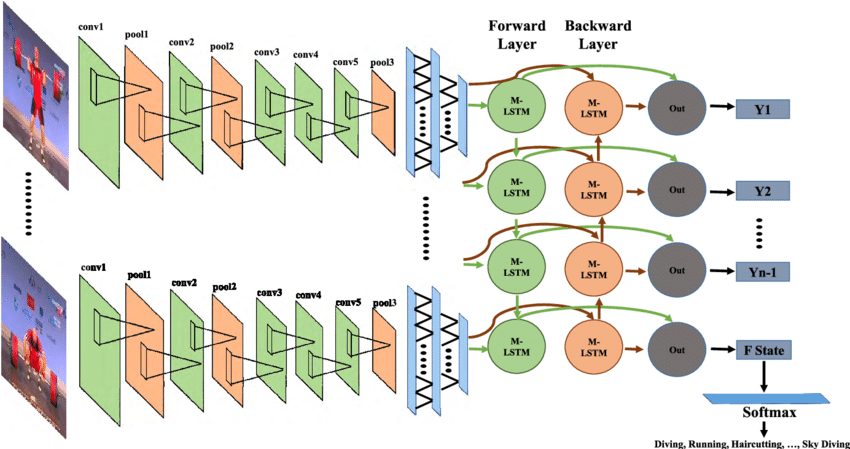
\includegraphics[width=1.00\columnwidth]{figures/lstm.png}
  \caption{The LSTM approach to sequentially process images.}~\label{fig:figure2}
\end{figure*}



 \section{Proposed Solution}
  \begin{figure*}
  \centering
  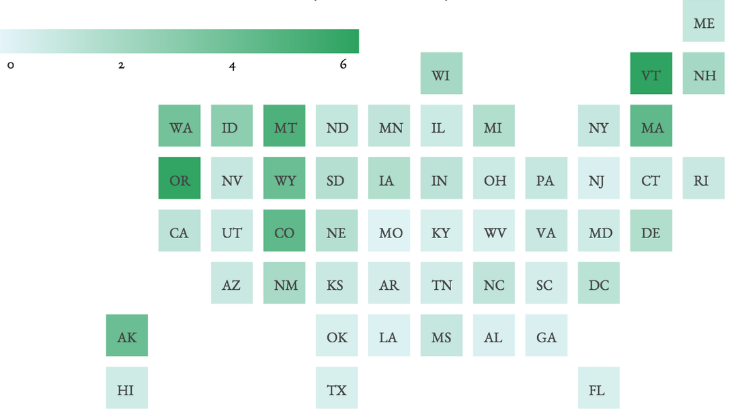
\includegraphics[width=1.00\columnwidth]{figures/mapGrids.png}
  \caption{The map of the US split up into grids the size of states and the soft maxed output on predictions of which grid the image came from.}~\label{fig:figure3}
\end{figure*}
 The proposed solution takes the following steps:
 \begin{itemize}
    \item The first step involves the map and defining geographic girds to collect data from. For this project the map of the United States will be chosen. This is because the country has a diverse geographic landscape with definitive features in each region. This can be leveraged by the CNN to give good results. Another reason for this choice is because a plethora of street view images are available for most regions in the country. Confining the area to just the united states will also make comprehensive training possible as using data from the entire planet will require a lot more computing power for training than is available for this project.
    \item The next step is to split the map into logical grids. The size of these grids will be a hyper-parameter to be tuned. A view of the US map split up into grids that are the size of states is show in Figure~\ref{fig:figure3}. The map will be split up into grids using google S2 geometry \cite{S2-geometry:Online}. Data points will then be scraped from each grid with the number of data points being scraped being a hyper parameter.
     \item Data will be scraped from google street view. This will be done using the google street view API \cite{Google-Street-veiw:Online}. Data scraped from a single location will act as a data point. Since google offers a 360 degree street view, multiple images will be taken at each location to act as a single data point for training. This list of images will be processed sequentially using the LSTM technique mentioned above.
     \item Once the data collection pipeline is ready, training will be conducted using three machine learning techniques mentioned in the related work section. As the first technique involving K-NN's is unsupervised, an extremely large training set will not be needed. The computational power required will be low as there will be no training required for the unsupervised approach. 
     \item The next technique involves using single images in  training a CNN. After training, given a test image, the CNN will have to produce a soft maxed output across grids of locations Figure~\ref{fig:figure3}. The training of this network will be computationally heavy. To make training efficient the network will be trained in batches with images being scraped during training. Google Colab GPU's will most likely be used for training.
      \item The final solution involves using a CNN/LSTM combination. Here a single training epoch will consist of multiple images obtained from a single 360 degree sweep of a location. The number of images collected from a single location will be a hyper-parameter. The list of images collected from a single location are processed sequentially using the CNN/LSTM logic mentioned in the related work section. The output will be a softmax across the grid of locations across the map. To make training efficient the network will be trained in batches with images being scraped during training. Google Colab GPU's will most likely be used for training.
 \end{itemize}
 
 \section{Evaluation}
  \begin{figure*}
  \centering
  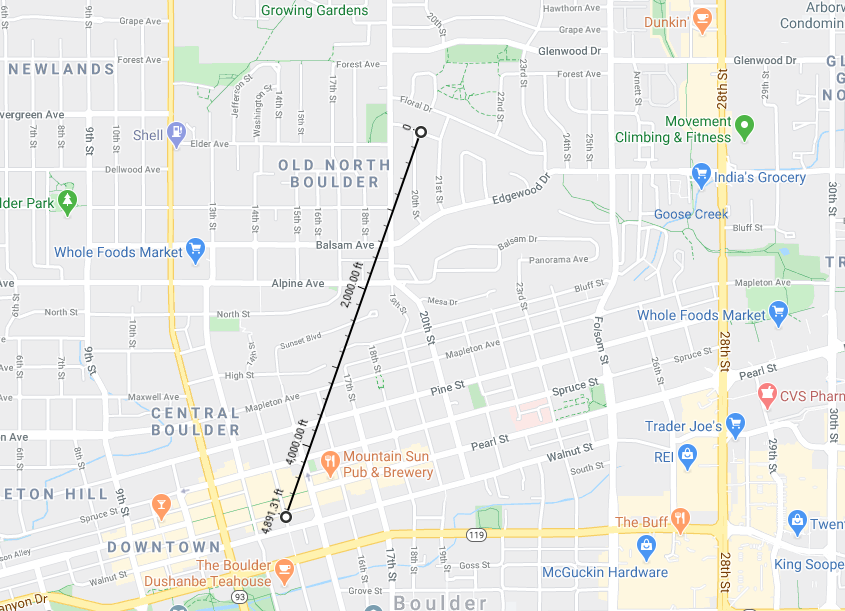
\includegraphics[width=0.7\columnwidth]{figures/evals.png}
  \caption{Using distance as an evaluation metric.}~\label{fig:figure4}
\end{figure*}
 The evaluation for the project will be done based on the euclidean distance (see Figure~\ref{fig:figure4}) between the predicted location grid and the actual location. The test set will be processed using the above mentioned machine learning techniques to get the softmaxed output. The top N softmaxed outputs are considered. Here N will be a hyper parameter. Out of the top N, the one that gives the grid with the least euclidean distance from the target location will be chosen. This way the models can be evaluated with the euclidean distance across the test set being summed up. The model with the least sum will be considered the best. Human player scores will be used as baselines to compare with model scores.


% BALANCE COLUMNS
\balance{}

% REFERENCES FORMAT
% References must be the same font size as other body text.

% \bibliographystyle{unsrt}
\bibliographystyle{SIGCHI-Reference-Format}
\bibliography{sample}

\end{document}

%%% Local Variables:
%%% mode: latex
%%% TeX-master: t
%%% End:
